\section{Analysis}

\begin{frame}{Analysis: Effect of Exploration}
\begin{figure}
    \centering
    \begin{subfigure}{\textwidth}
        \centering
        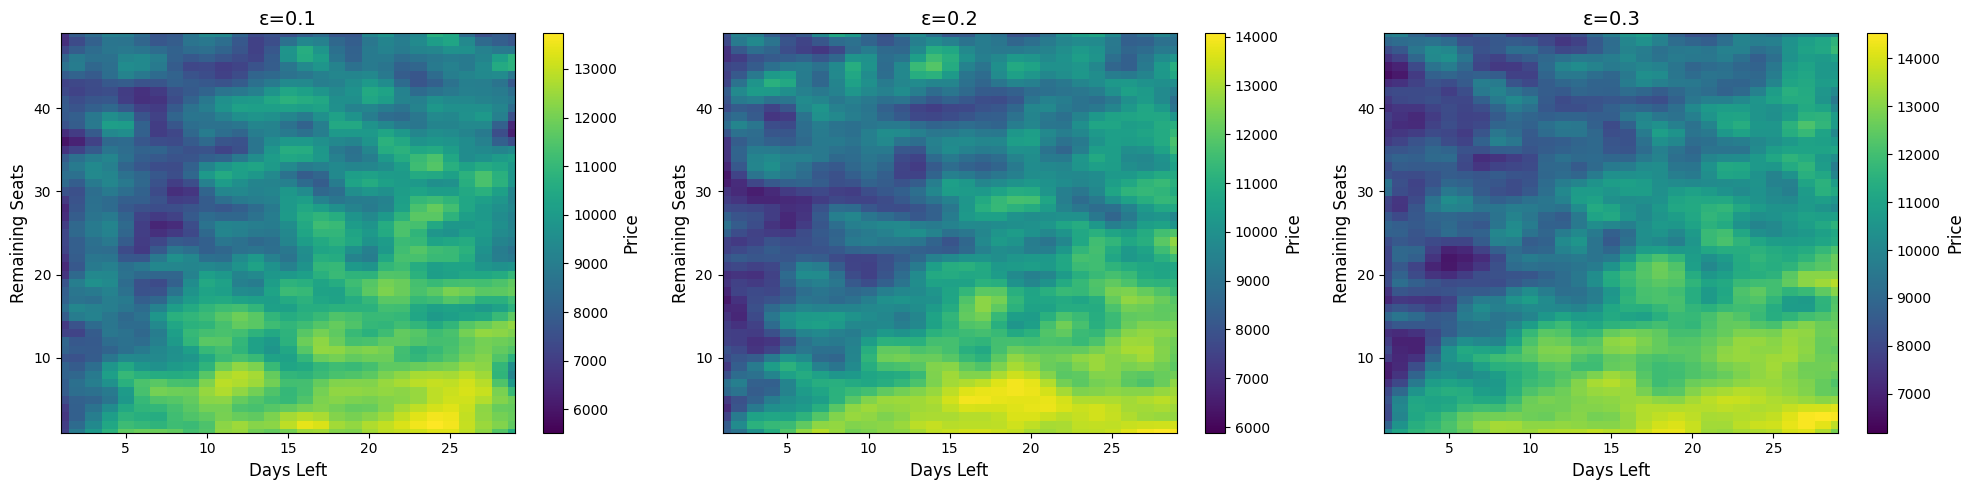
\includegraphics[width=\textwidth]{epsilon_policy.png}
        \caption{Learned Policy}
    \end{subfigure}
    \begin{subfigure}{\textwidth}
        \centering
        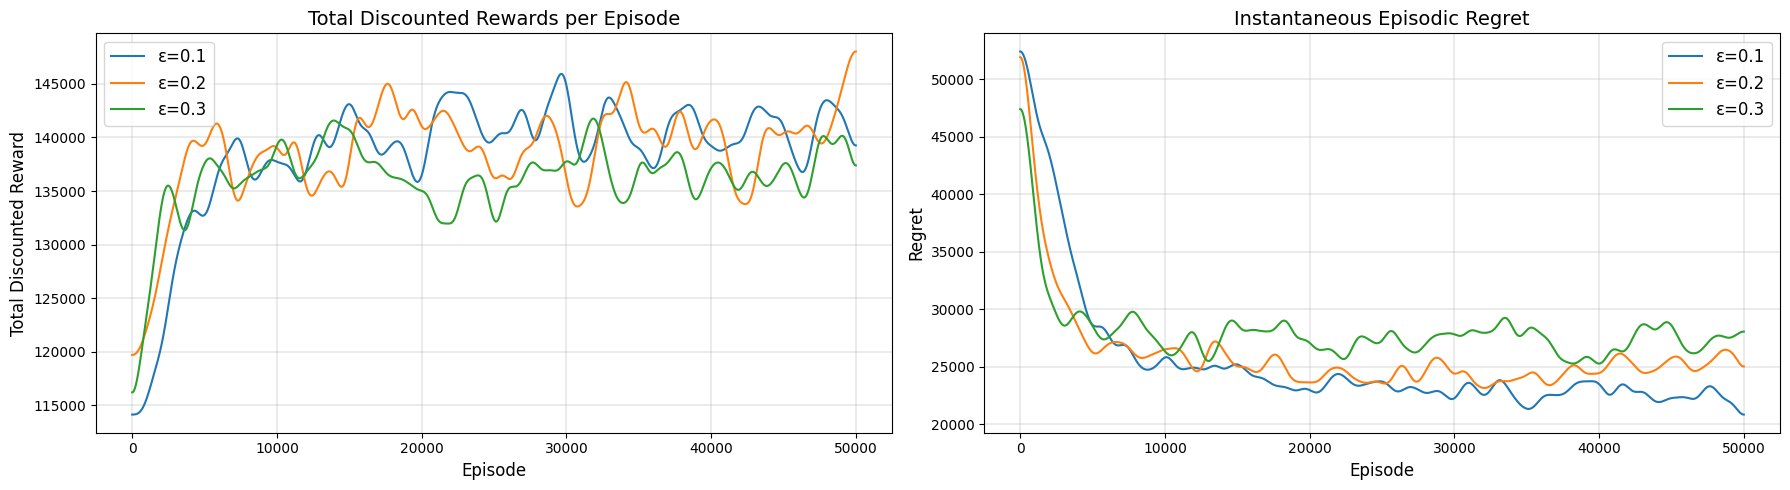
\includegraphics[width=0.9\textwidth]{epsilon_metrics.png}
        \caption{Episodic Rewards and Regrets}
    \end{subfigure}
    \caption{Q-Learning at different levels of $\epsilon-$greedy Exploration}
\end{figure}
\end{frame}

\begin{frame}{Analysis: Effect of Trace Decay}
\begin{figure}
    \centering
    \begin{subfigure}{\textwidth}
        \centering
        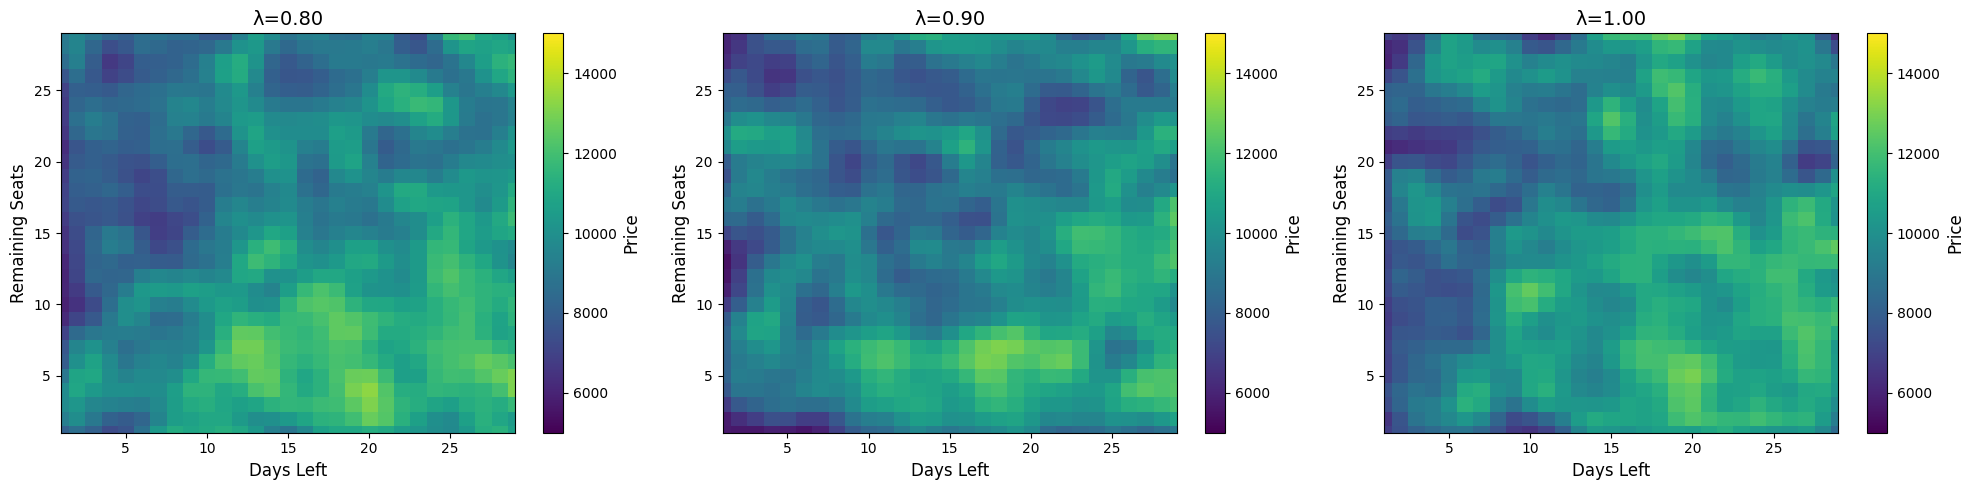
\includegraphics[width=\textwidth]{lambda_policy.png}
        \caption{Learned Policy}
    \end{subfigure}
    \begin{subfigure}{\textwidth}
        \centering
        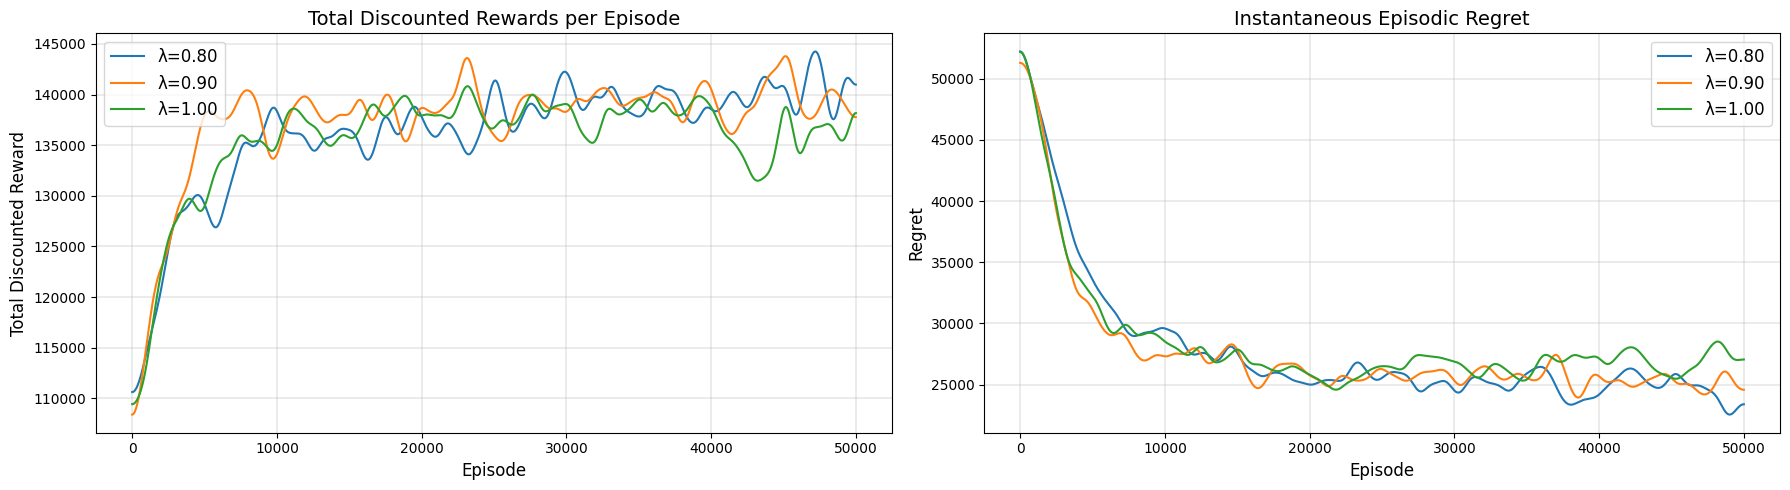
\includegraphics[width=0.9\textwidth]{lambda_metrics.png}
        \caption{Episodic Rewards and Regrets}
    \end{subfigure}
    \caption{SARSA($\lambda$) at different levels of Trace Decay}
\end{figure}
\end{frame}

\begin{frame}{Conclusion}
\begin{itemize}
    \setlength\itemsep{1.5em}
    \item Learned policies lacked similarity in close neighbourhood, contrary to our intuitive understanding.
    \item Convergence rate was similar in Q-Learning and SARSA($\lambda$). However, Q-Learning got closer to the optimal policy and acquired less regret.
    \item Higher exploration improved the policy and speed of convergence, but resulted in more regret.
    \item Policies learned with smaller trace decay (higher $\lambda$) appeared to be closer to the optimal policy. However, the effect was not very prominent.
\end{itemize}
\end{frame}
